\begin{frame}{Machine learning in turbomachinery}
    \begin{block}{Task}
        Due to the \textbf{non stochastic nature} of the problem. This analysis will be based on a \textbf{regression}: 
        \begin{equation*}
            \mathnormal{f}: \mathcal{X} \rightarrow \mathcal{Y}
        \end{equation*}
    \end{block}
    \begin{block}{Training \& Test}
        \vspace{-0.5cm}
        \begin{align*}
            \boldsymbol{x_*}, \boldsymbol{x_{**}} \in \mathcal{X} \\
            \boldsymbol{y_*}, \boldsymbol{y_{**}} \in \mathcal{Y}
        \end{align*}
    \end{block}
    \begin{block}{Regression modeling}
        \begin{equation*}
            \boldsymbol{y} \approx \hat{\mathnormal{f}}(\boldsymbol{x}, \boldsymbol{w}), \text{ where } \boldsymbol{w} \in \mathcal{W}
        \end{equation*}
    \end{block}
\end{frame}

\begin{frame}{Minimization \& testing}
    \begin{block}{Error analysis}
        In order to understand the performance of the approximated $\mathnormal{f}$, $\hat{\mathnormal{f}}$, it is necessary to setup a performance parameter:
        \begin{equation*}
            J_{(\boldsymbol{x})} = \frac{1}{m} \sum^{m-1}_{j = 0} \big( \hat{\mathnormal{f}}_{(\boldsymbol{x}_j, \boldsymbol{w})} - \boldsymbol{y}_j\big)^2
        \end{equation*}
    \end{block}
    \vspace{-0.5cm}
    \begin{columns}
        \column{0.55\textwidth}
        \begin{block}{$\boldsymbol{w}$ computation}
            \begin{equation*}
                min \Bigg( J_{(\boldsymbol{x_*})} = \frac{1}{m_*} \sum^{m_* - 1}_{j = 0} \big( \hat{\mathnormal{f}}_{(\boldsymbol{x_*}_j, \boldsymbol{w})} - \boldsymbol{y_*}_j\big)^2 \Bigg)
            \end{equation*}
        \end{block}
        \column{0.55\textwidth}
        \begin{block}{$\boldsymbol{w}$ testing}
            \begin{equation*}
                J_{(\boldsymbol{x_{**}})} = \frac{1}{m_{**}} \sum^{m_{**} - 1}_{j = 0} \big( \hat{\mathnormal{f}}_{(\boldsymbol{x_{**}}_j, \boldsymbol{w})} - \boldsymbol{y_{**}}_j\big)^2
            \end{equation*}
        \end{block}
    \end{columns}
\end{frame}

\begin{frame}{Radial Basis Functions}
    \begin{block}{$\hat{\mathnormal{f}}$ definition}
        \vspace{-0.5cm}
        \begin{align*}
            \mathnormal{f} \approx \hat{\mathnormal{f}} & = \boldsymbol{\Phi}_{(\boldsymbol{x})} \cdot \boldsymbol{w} \\
            \boldsymbol{y} \approx \hat{\mathnormal{f}}_{(\boldsymbol{x}, \boldsymbol{w})} & = \boldsymbol{\Phi}_{(\boldsymbol{x})} \cdot \boldsymbol{w} \\ 
            \boldsymbol{\Phi}_{(\boldsymbol{x})} & = 
            \begin{bmatrix}
                \lvert &  & \lvert \\ 
                \Phi_{0_{ ( \boldsymbol{x}, \ \boldsymbol{p}_0 ) } } & ... & \Phi_{n_{ ( \boldsymbol{x}, \ \boldsymbol{p}_n ) } } \\
                \lvert &  & \lvert 
            \end{bmatrix}
        \end{align*}
    \end{block}
    \vspace{-0.5cm}
    \begin{columns}
        \column{0.5\textwidth}
        \begin{block}{Gaussian RBF model}
            \vspace{-0.5cm}
            \begin{align*}
                d_j (\boldsymbol{x}) & = \lvert \boldsymbol{x} - \boldsymbol{x}^*_j \lvert \\
                \Phi_{j_{ ( \boldsymbol{x}, \ \boldsymbol{x}^*_j, \ c_j )}} & = exp \big( -c^2_j \ d_j (\boldsymbol{x})^2 \big) 
            \end{align*}
        \end{block}
        \column{0.5\textwidth}
        \vspace{-0.57cm}
        \begin{figure}
            \centering
            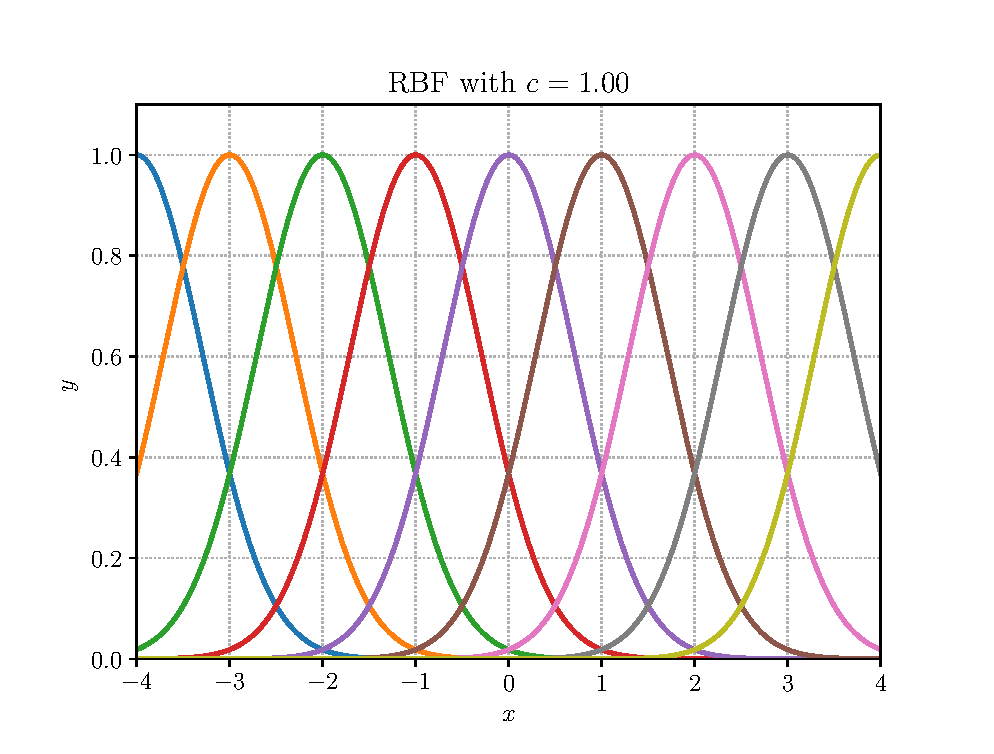
\includegraphics[scale=0.27]{./images/RBF.eps}
        \end{figure}
    \end{columns}
\end{frame}

% \begin{frame}{Data distribution}
%     \begin{figure}
%         \centering
%         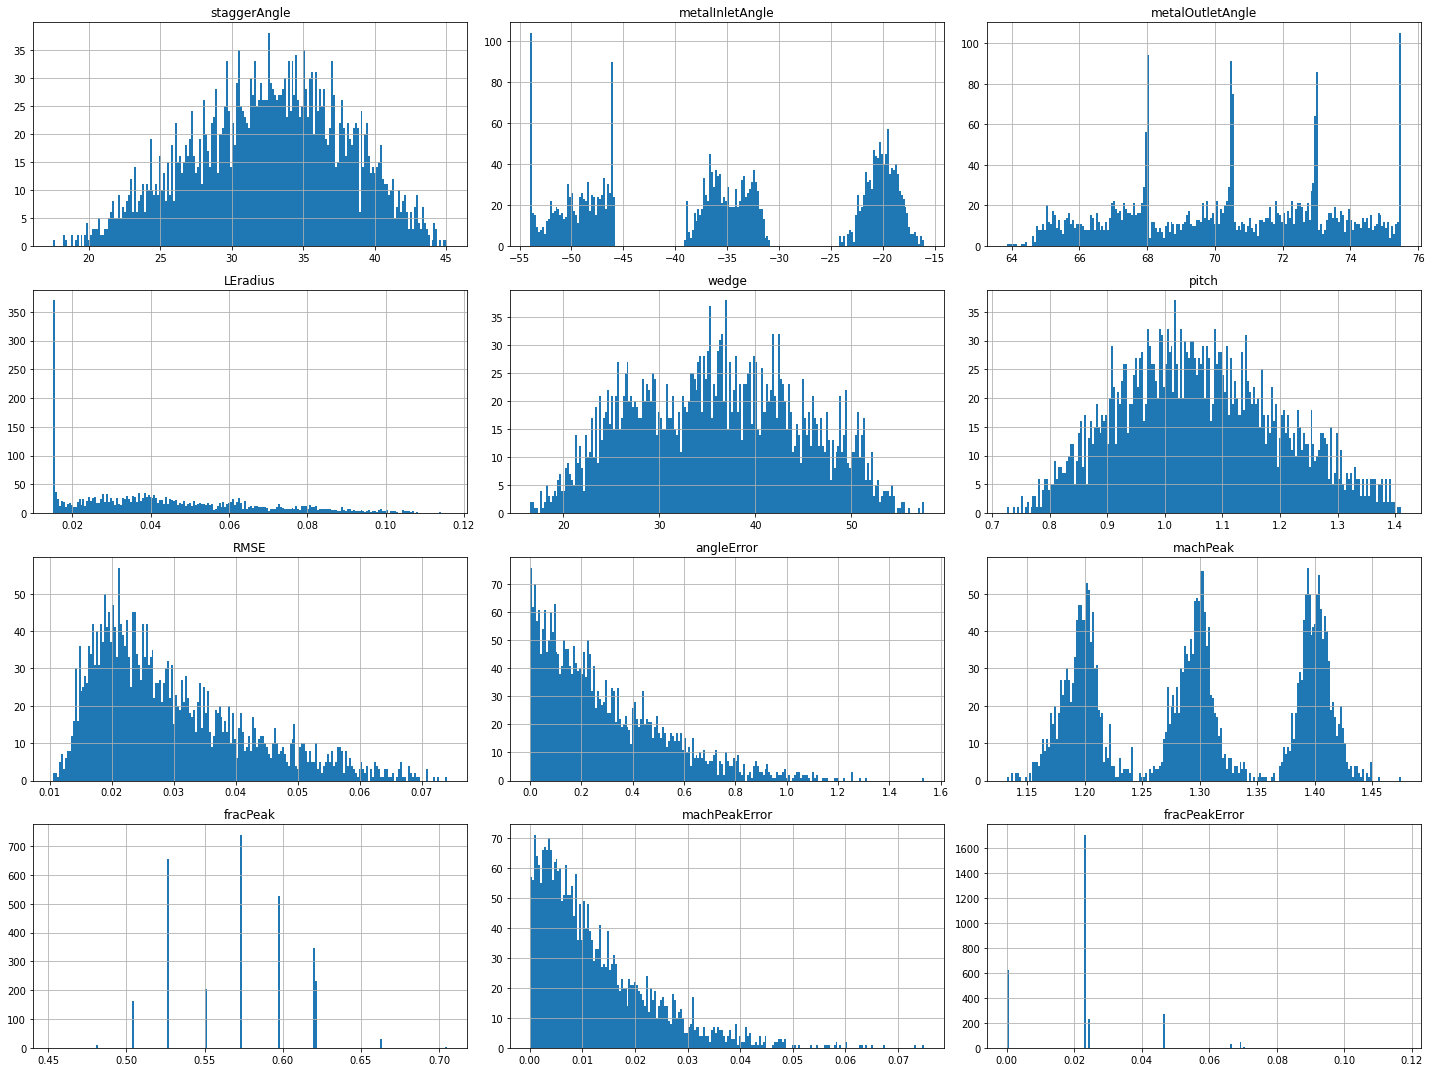
\includegraphics[scale=0.19]{./images/histGrid.png}
%     \end{figure}
% \end{frame}

% \begin{frame}{Data analysis}
%     \begin{figure}
%         \centering
%         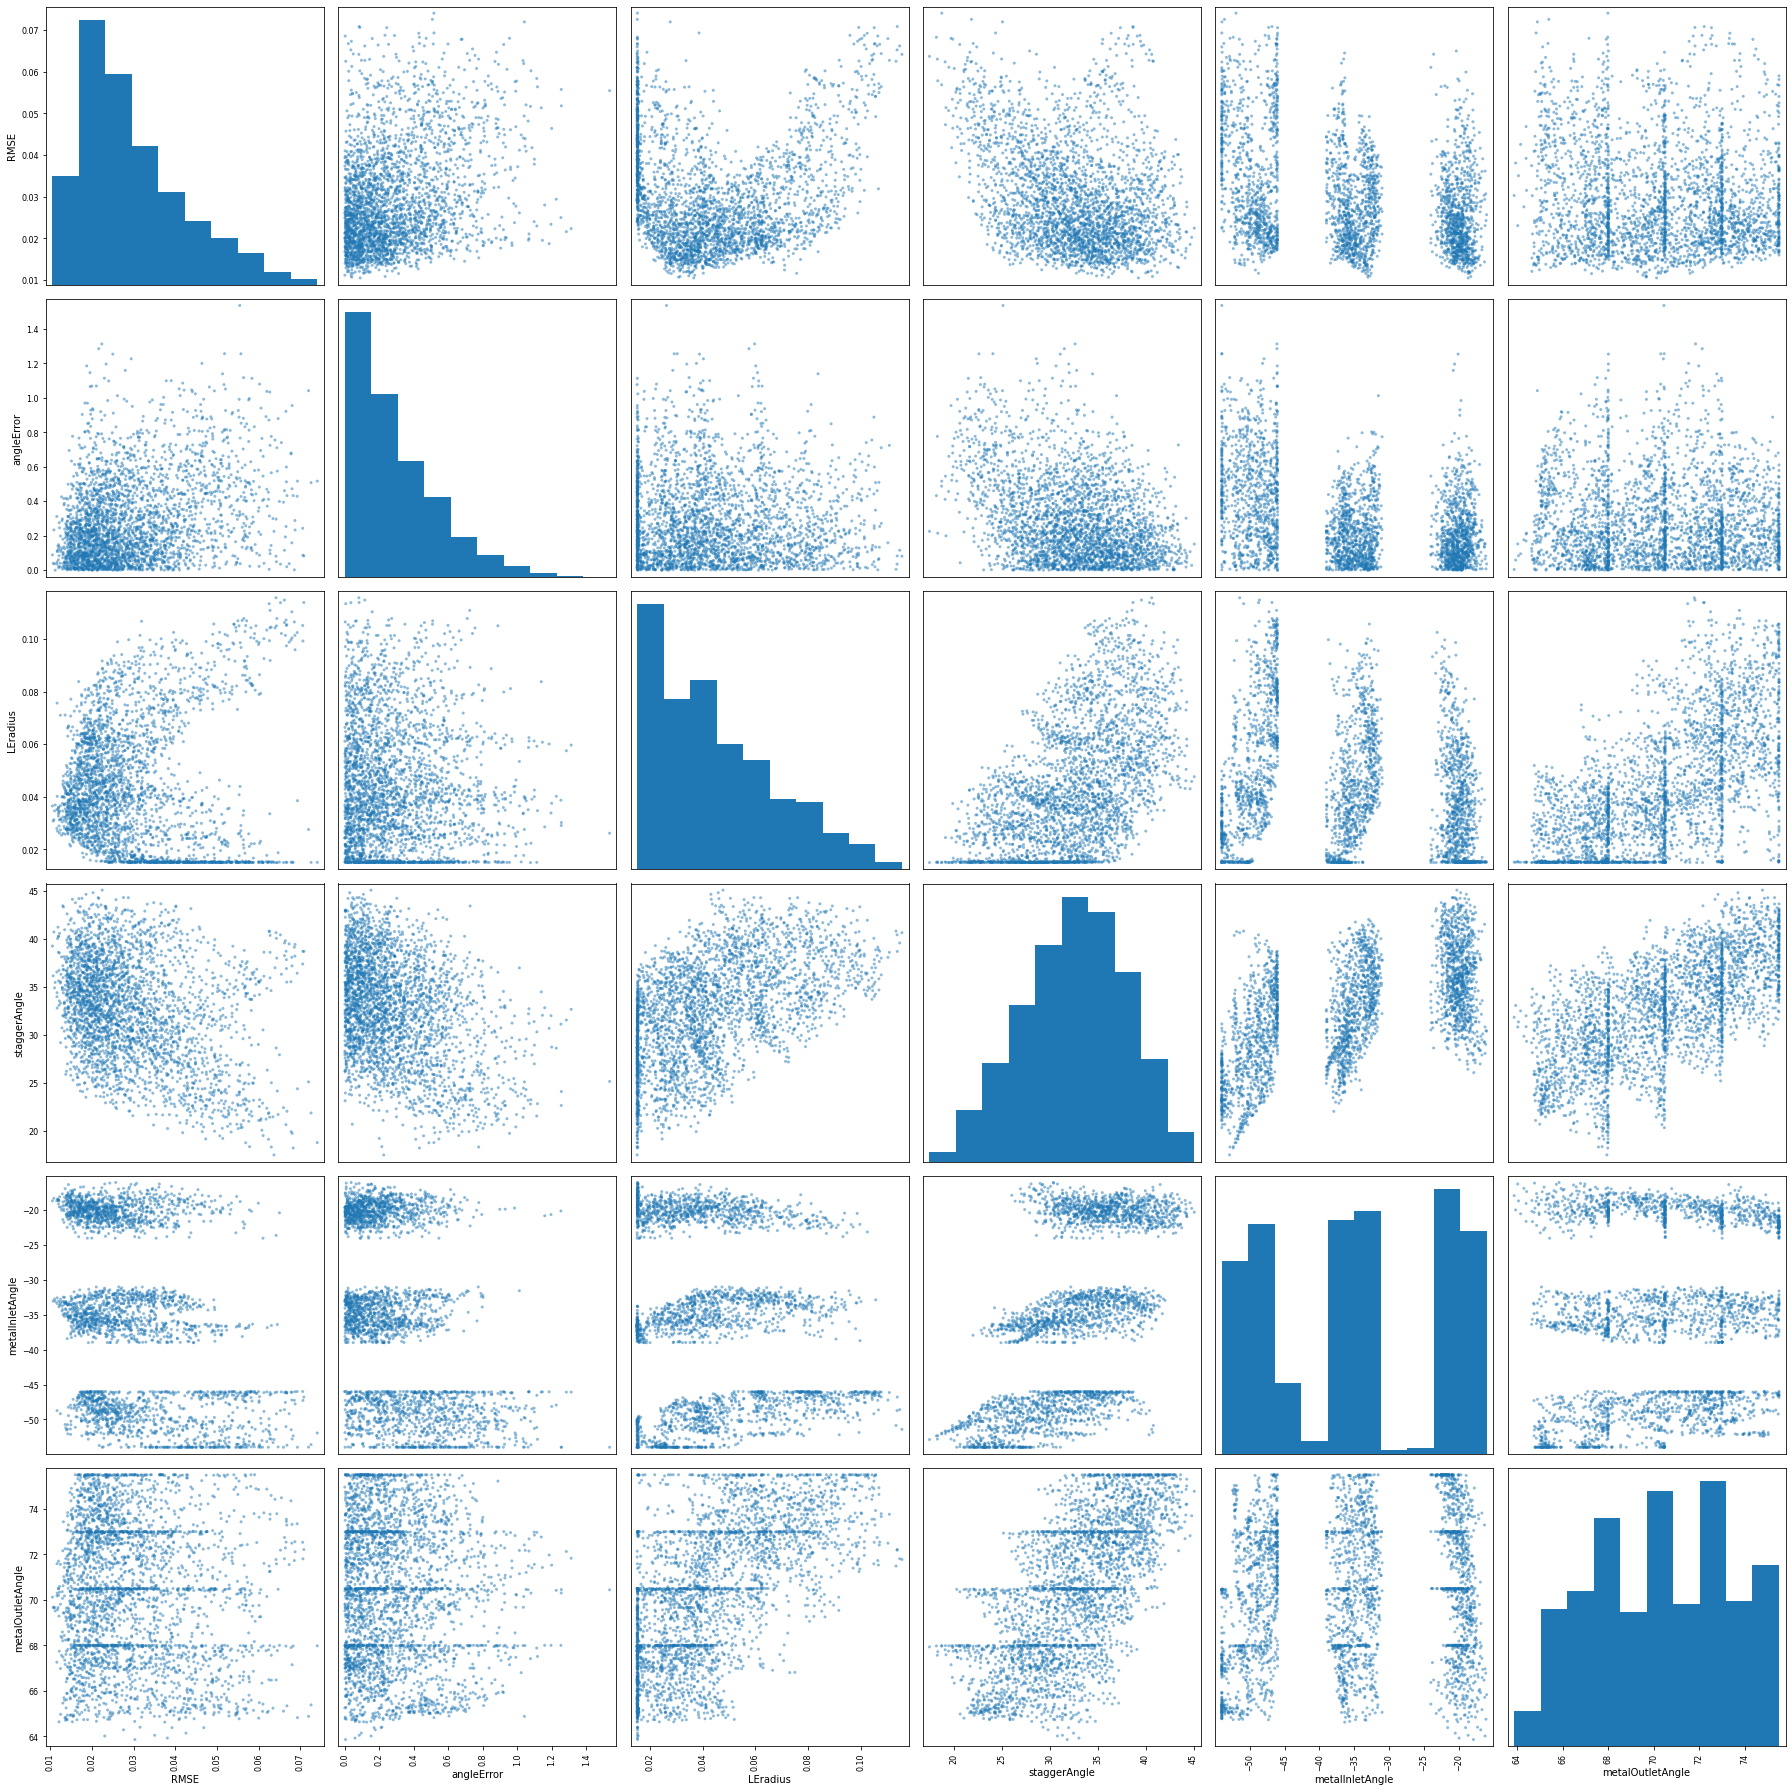
\includegraphics[scale=0.115]{./images/correlationGrid.png}
%     \end{figure}
% \end{frame}

\begin{frame}{RBF interpolation}
    \vspace{-0.8cm}
    \begin{columns}
        \column{0.5\textwidth}
        \lstinputlisting[style=customPy, firstline=1, lastline=12, caption=Data preprocessing]{codes/ML.txt}
        \column{0.5\textwidth}
        \lstinputlisting[style=customPy, firstline=14, lastline=26, caption=RBF interpolation]{codes/ML.txt}
    \end{columns}
    \vspace{-0.8cm}
    \begin{columns}
        \column{0.5\textwidth}
        \lstinputlisting[style=customPy, firstline=27, caption=RBF scoring]{codes/ML.txt}
        \column{0.5\textwidth}
        \vspace{0.8cm}
        \begin{figure}
            \centering
            
\includegraphics[scale=0.5]{./images/scikitLogo.png}
        \end{figure}
    \end{columns}
\end{frame}

\begin{frame}{Principal Component Analysis}
    \begin{columns}
        \column{0.5\textwidth}
            \vspace{1cm}
            \begin{block}{Dimensionality reduction}
                Identify the modes which account the most amount of variance in the dataset.
                \begin{align*}
                    \boldsymbol{X} & = \boldsymbol{U} \ \boldsymbol{\Sigma} \ \boldsymbol{V}^T \\
                    \boldsymbol{V} & = 
                        \begin{bmatrix}
                            \lvert & & \lvert \\
                            \boldsymbol{c}_0 & ... & \boldsymbol{c}_n \\ 
                            \lvert & & \lvert  
                        \end{bmatrix} 
                \end{align*}
            \end{block}
        \column{0.5\textwidth}
            \lstinputlisting[style=customPy, caption=PCA]{codes/PCA.txt}
            \vspace{-0.2cm}
            \begin{figure}
                \centering
                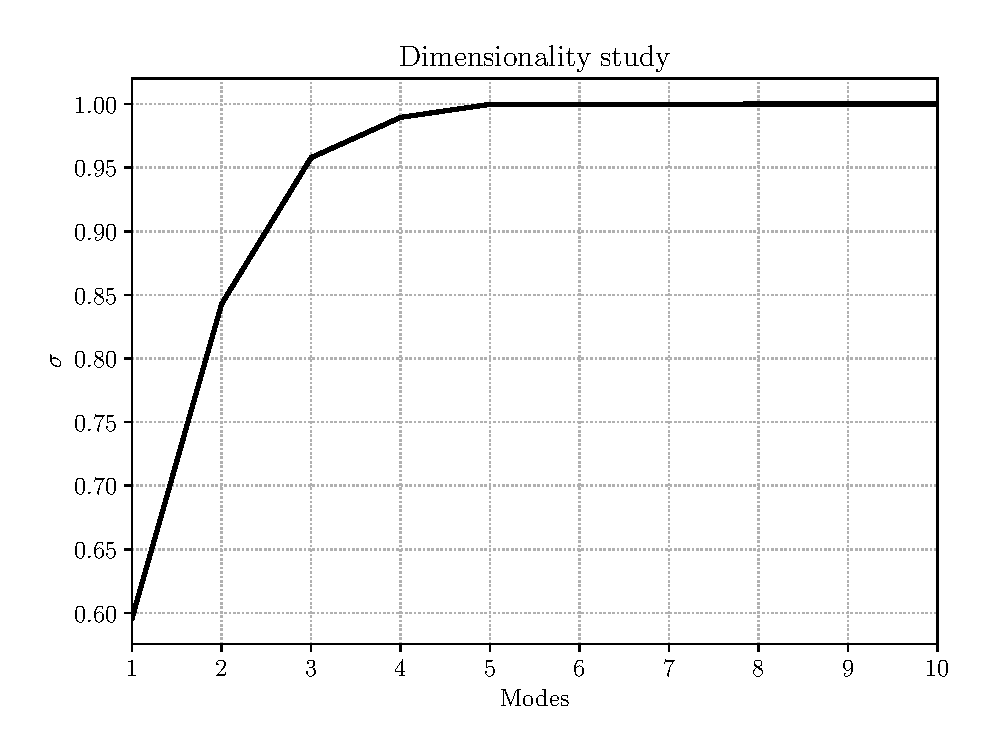
\includegraphics[scale=0.25]{./images/PCAmodes.eps}
            \end{figure}
    \end{columns}
\end{frame}

% \begin{frame}{Radial Basis Function}
%     \begin{block}{ML algorithm}
%         The interpolation of data is made using the radial basis function network. 
%         \newline 
%         This method allows to interpolate without any error the database entries and to interpolate with some error the other domain points.
%     \end{block}
%     \begin{alertblock}{ML entries and errors filtering}
%         Since the database has errors coming from the blade optimization process (expecially on the exit flow angles $\alpha_2$), 
%         the blade will be input inside the optimization algorithm using a target exit flow angle of $\alpha_{2, target} + \Delta \alpha_2$. 
%         \newline 
%         This way of studying will guarantee an study point that tracks smoothly the target load and has an exit flow angle error close to zero ($\Delta \alpha_2 \approx 0$).
%         \newline 
%         Once the fist data fitting is made, a study on the corner points will be made in order to make better prediction of a new optimization point for the optimization algorithm.
%     \end{alertblock}
% \end{frame}
